\documentclass[aps,pra,reprint,superscriptaddress,nofootinbib,floatfix]{revtex4-2}

\usepackage{amsmath,amssymb,amsthm,bm}
\usepackage{booktabs}
\usepackage{graphicx}
\usepackage{microtype}
\usepackage{xcolor}
\usepackage[colorlinks=true,linkcolor=blue,citecolor=blue,urlcolor=blue]{hyperref}

\newcommand{\Cl}{\mathrm{Cl}}
\newcommand{\C}{\mathbb{C}}
\newcommand{\R}{\mathbb{R}}
\newcommand{\Tr}{\operatorname{Tr}}
\newcommand{\ii}{\mathrm{i}}
\newcommand{\ket}[1]{\lvert #1\rangle}
\newcommand{\bra}[1]{\langle #1\rvert}
\newcommand{\avg}[1]{\langle #1\rangle}
\newcommand{\calP}{\mathcal{P}}
\newcommand{\calW}{\mathcal{W}}
\newcommand{\supp}{\operatorname{supp}}
\newcommand{\sgn}{\operatorname{sgn}}
\newcommand{\Var}{\operatorname{Var}}

\newtheorem{lemma}{Lemma}
\newtheorem{proposition}{Proposition}
\newtheorem{corollary}{Corollary}

\begin{document}

\title{Confidence-certified, measurement-efficient operator selection for ADAPT-VQE in an operator-centric Clifford algebra}

\author{Ginanjar Utama}
\email{ginanjar.utama@gmail.com}
\affiliation{Department of Engineering Physics, Institut Teknologi Bandung, Bandung, Indonesia}

\author{Hermawan Kresno Dipojono}
\email{dipojono@itb.ac.id}
\affiliation{Department of Engineering Physics, Institut Teknologi Bandung, Bandung, Indonesia}

\date{\today}

\begin{abstract}
Adaptive variational eigensolvers grow a circuit by repeatedly selecting the pool operator with the largest energy gradient, but on hardware that ranking must be inferred from finite measurements, and a wrong ranking commits the ansatz before optimization begins. We develop a measurement-efficient, statistically certified selection framework in a sparse operator-centric realization of the complex Clifford algebra $\Cl(2n,\C)\cong M(2^n,\C)$. All commutator-gradient selection observables $G_j=-\tfrac{\ii}{2}[H,P_j]$ are represented collectively in one sparse candidate-by-word coefficient matrix over the shared Pauli-word set $\calW=\bigcup_j\supp(G_j)$, so every candidate estimate is a linear reconstruction from a single cumulative measurement cache; qubit-wise-commuting (QWC) grouping then collapses that cache to one circuit per group. A best-arm selector reports one of four explicit outcomes---resolved, near-optimal, below-threshold, or budget-exhausted-ambiguous---using simultaneous confidence bounds with a user-set error budget, and never silently returns an unresolved maximum. On five transverse-field Ising and random-field Ising families at $n=4$ (100 seeds), certified selection reaches median relative energy errors between $10^{-5}$ and machine precision at a fixed operator budget, two to more than three orders of magnitude below random selection; QWC grouping cuts the distinct measurement circuits by $3.1$--$4.0\times$ at unchanged accuracy; and variance-proportional shot allocation reduces the ambiguous-selection rate by $26$--$49\%$. On molecular Hamiltonians the framework exposes a sharp proxy-versus-gradient boundary: a FAST-inspired determinant-population proxy reaches chemical accuracy roughly $400\times$ more cheaply than certified gradient selection on equilibrium H$_2$, LiH, and BeH$_2$, but fails deterministically on the correlated H$_4$ chain ($56$~mHa, worse than random selection), where gradient selection still converges. We further report a negative result: classically optimized stabilizer initialization does not reduce the non-Clifford correction that adaptive selection must supply. We claim no asymptotic speedup over matrix methods; the contribution is a reproducible, algebraically unified account of when finite-shot adaptive selection can be certified and when it cannot.
\end{abstract}

\maketitle

\section{Introduction}
\label{sec:intro}

The variational quantum eigensolver (VQE) pairs a parameterized state with a classical optimizer to approximate low-energy eigenstates \cite{peruzzo2014vqe,mcclean2016theory}. Adaptive variants such as ADAPT-VQE grow the ansatz operator by operator, appending at each step the pool generator with the largest instantaneous energy gradient \cite{grimsley2019adapt,tang2021qubitadapt}. Analytic circuit gradients remove finite-difference bias \cite{mitarai2018qcl,schuld2019gradients,wierichs2022general}, but adaptation relocates the difficulty: the pool gradients must themselves be \emph{ranked} from finite measurements, and because a selection permanently fixes the next ansatz slot before any parameter is optimized, a ranking error is not refunded by later reoptimization \cite{scriva2024challenges}. This selection step, not parameter optimization, is the object of the present paper.

Several lines of work attack the measurement cost of selection from complementary directions. Anastasiou \emph{et al.} reduce the number of distinct commuting gradient measurements \cite{anastasiou2023gradients}; the FAST theory of Majland \emph{et al.} replaces commutator gradients by a sampled determinant-population proxy for fermionic chemistry \cite{majland2023fast}; Long \emph{et al.} use layering and subpool exploration to cut processor calls and depth \cite{long2024layering}; and Ikhtiarudin \emph{et al.} reuse Pauli outcomes across candidates and allocate shots by variance \cite{ikhtiarudin2025shot}. What has been missing is a selection procedure that (i) estimates the \emph{exact} commutator gradient rather than a proxy, (ii) reuses every shared measurement globally across the pool, and (iii) attaches an explicit, user-controlled probability that the chosen operator is correct---so that ``the measurement budget was exhausted without resolving the ranking'' is a reported outcome rather than a silent guess.

We provide such a procedure inside a sparse operator-centric realization of the complex Clifford algebra $\Cl(2n,\C)\cong M(2^n,\C)$ \cite{somaroo1998operations,hrdina2022clifford,silva2025operator}, in which states, gates, observables, channels, and selection gradients are all elements of one Pauli-word algebra. The algebraic foundation---the phase-consistent Pauli-word/Clifford-blade dictionary, the distinction between Pauli-word rotations and Spin rotors, and the exact transpose-parity rule that eliminates the even-$Y$ candidate sector for real Hamiltonians---is developed in a companion manuscript \cite{utama2025operatorcentric}; Sec.~\ref{sec:foundation} recalls only what the selection framework needs. The contribution of the present work is fourfold:
\begin{enumerate}
    \item a \emph{global commutator bank} that stores all selection observables in one sparse candidate-by-word matrix, so estimates and variances of every candidate are reconstructed from a single measurement cache (Sec.~\ref{sec:bank});
    \item shared-word cumulative caching and qubit-wise-commuting grouping, which pay for each Pauli word once per allocation round and collapse the cache to one circuit per commuting group (Sec.~\ref{sec:grouping});
    \item a best-arm selector with simultaneous confidence bounds and a four-way explicit outcome, controlling the probability of selecting the wrong operator (Sec.~\ref{sec:confidence});
    \item a 100-seed, multi-family, and molecular study that measures selection quality, circuit cost, and the exact boundary at which a determinant-population proxy fails while gradient selection does not (Sec.~\ref{sec:results}).
\end{enumerate}

We benchmark on the open and periodic transverse-field Ising model (TFIM),
\begin{equation}
H(J,h)=-J\sum_{\langle j,k\rangle}Z_jZ_k-h\sum_{j}X_j,
\label{eq:tfim}
\end{equation}
whose critical point is $h/J=1$ \cite{pfeuty1970ising}; a random-field Ising ensemble; the XXZ chain; and the molecules H$_2$, LiH, BeH$_2$, and the H$_4$ chain. All numerical claims are bounded to $n\le6$ (spin) and four-qubit-scale active spaces (chemistry); we claim correctness and qualitative behavior, not favorable asymptotic scaling.

\section{Operator-centric selection observables}
\label{sec:foundation}

\subsection{One algebra for gradients and measurements}

Let $\gamma_0,\dots,\gamma_{2n-1}$ generate $\Cl(2n,\C)$ with $\gamma_a\gamma_b+\gamma_b\gamma_a=2\delta_{ab}\mathbf 1$; the standard irreducible representation gives $\Cl(2n,\C)\cong M(2^n,\C)$. Every $n$-qubit operator is stored sparsely in the Hermitian Pauli-word basis $\calP_n=\{I,X,Y,Z\}^{\otimes n}$,
\begin{equation}
A=\sum_{W\in\calP_n}a_W\,W,\qquad \Tr(A^\dagger B)=2^n\!\sum_W a_W^*b_W,
\label{eq:pauliexp}
\end{equation}
with the Jordan--Wigner strings $\gamma_{2j}=Z_0\cdots Z_{j-1}X_j$, $\gamma_{2j+1}=Z_0\cdots Z_{j-1}Y_j$ providing the exact bridge from anticommuting Clifford generators to local Paulis \cite{jordan1928,utama2025operatorcentric}. Density operators, unitaries, Hermitian observables, and Kraus maps are all elements of Eq.~\eqref{eq:pauliexp}; crucially for what follows, so is every ADAPT selection gradient. The advantage exploited here is not expressivity---$\Cl(2n,\C)$ and $M(2^n,\C)$ are isomorphic---but \emph{uniformity}: a candidate's exact gradient, its finite-shot estimator, and its uncertainty are the same typed object, and shared structure between candidates is visible as shared Pauli words.

\subsection{The selection observable and the odd-$Y$ sector}
\label{sec:oddy}

Appending a candidate rotation $R_P(\theta)=e^{-\ii\theta P/2}$ to the current state $\rho$ has initial energy slope
\begin{equation}
g_P=\left.\partial_\theta \Tr\!\left[HR_P(\theta)\rho R_P^\dagger(\theta)\right]\right|_{\theta=0}=\Tr(G_P\,\rho),\quad G_P=-\tfrac{\ii}{2}[H,P],
\label{eq:gp}
\end{equation}
with $G_P=G_P^\dagger$. Ranking candidates therefore requires no candidate-specific shifted circuits: it requires the current state and the expectation values of the Pauli words appearing in the Hermitian observables $\{G_P\}$. A single structural fact prunes half of the pool exactly. Writing $\nu_Y(W)$ for the number of $Y$ factors in $W$, computational-basis transposition acts as $W^T=(-1)^{\nu_Y(W)}W$, and one has the following \cite{utama2025operatorcentric}.

\begin{proposition}[Transpose-parity selection rule]
\label{prop:oddy}
Let $H$ and $\rho$ be real symmetric. If a Hermitian Pauli word $P$ has even $\nu_Y(P)$, then $\Tr(\rho[H,P])=0$, so $g_P=0$. Moreover, an odd-$Y$ rotation preserves real symmetry, so for a real reference and an odd-$Y$ ansatz every even-$Y$ candidate has zero gradient at every step.
\end{proposition}

Consequently the pool may be restricted to odd-$Y$ words with \emph{no change} to the exact ADAPT trajectory, only a smaller candidate and observable count. This restriction is the first, exact, layer of measurement reduction, and it holds for every real Hamiltonian in this study; it is an algebraic pool symmetry, distinct from---though in the same spirit as---the symmetry-preserving ansatz constructions of Refs.~\cite{yoo2025symmetry} and the explicit Clifford transformations of fermionic operators developed for many-body computation \cite{evangelista2025exact,magoulas2026clifford}. We verify it numerically in Sec.~\ref{sec:results} by confirming that odd-$Y$-restricted and unrestricted pools produce identical exact trajectories.

\section{Measurement-efficient certified selection}
\label{sec:method}

\subsection{Global commutator bank}
\label{sec:bank}

For a pool $\{P_j\}_{j=1}^{m}$ and a real Hamiltonian $H=\sum_w h_w W_w$, each selection observable expands as $G_j=\sum_{w} c_{jw}W_w$ with real coefficients $c_{jw}$ (Hermiticity of $G_j$ and reality of $H$). Rather than give each candidate its own accumulator, we form the union word set
\begin{equation}
\calW=\bigcup_{j}\supp(G_j)
\label{eq:wordset}
\end{equation}
once, and store the sparse candidate-by-word matrix $C=(c_{jw})$. The estimator of candidate $j$ is then a linear reconstruction from shared per-word means $\widehat m_w$,
\begin{equation}
\widehat g_j=\sum_{w\in\calW}c_{jw}\,\widehat m_w,\qquad
\widehat\Var(\widehat g_j)=\sum_{w}c_{jw}^2\,\widehat\Var(\widehat m_w),
\label{eq:bankest}
\end{equation}
computed against a single cache of measurements. Because pool generators differ by local dressing, the $G_j$ overlap heavily: across the TFIM and random-Ising pools the number of per-candidate word slots exceeds $|\calW|$ by a factor that grows with the pool, and every unit of that factor is a measurement the shared cache pays for once rather than $m$ times.

\subsection{Cumulative caching and QWC grouping}
\label{sec:grouping}

Within a selection step the state is fixed, so all rounds of measurement accumulate into one per-word cache of shot counts $N_w$ and $+1$-outcome counts $k_w$; escalation adds shots rather than discarding earlier samples, and reconstruction \eqref{eq:bankest} reads the running totals. To reduce the number of distinct \emph{circuits}, the words of $\calW$ (or of the currently active subset) are partitioned into qubit-wise-commuting (QWC) groups by greedy largest-degree-first coloring: two words qubit-wise commute when at every qubit their letters agree or one is the identity, so an entire group is diagonal in one product measurement basis and is read out by a single circuit. Sampling a group jointly from its rotated-basis computational distribution yields correlated per-word outcomes with the correct marginals, so grouping changes $N_{\text{circuits}}$ but not the estimator. This is the mechanism behind the circuit reductions in Sec.~\ref{sec:res-spin}.

\subsection{Simultaneous confidence bounds and the four-way outcome}
\label{sec:confidence}

We estimate per-word means with a Jeffreys pseudocount, $\widetilde p_w=(k_w+\tfrac12)/(N_w+1)$, $\widetilde m_w=2\widetilde p_w-1$, and $\widehat\Var(\widehat m_w)=(1-\widetilde m_w^2)/(N_w+1)$, so a finite sample of identical outcomes never yields zero estimated variance. Propagating through Eq.~\eqref{eq:bankest} gives $\widehat\Var(\widehat g_j)$, from which a two-sided normal radius at simultaneous level $1-\delta$ across the $m$ active candidates is
\begin{equation}
r_j=z_{1-\delta'/2}\,\sqrt{\widehat\Var(\widehat g_j)},\qquad
\delta'=1-(1-\delta)^{1/m},
\label{eq:radius}
\end{equation}
using the \v{S}id\'ak correction \cite{sidak1967rectangular} (Bonferroni is available and nearly identical here). The selector maintains simultaneous intervals $[\,|\widehat g_j|-r_j,\ |\widehat g_j|+r_j\,]$ and applies a best-arm identification rule \cite{evendar2006action,jamieson2014best}: the empirical leader $\hat\jmath$ is \emph{resolved} only when its lower bound exceeds every rival's upper bound,
\begin{equation}
|\widehat g_{\hat\jmath}|-r_{\hat\jmath}\;>\;\max_{k\neq\hat\jmath}\bigl(|\widehat g_k|+r_k\bigr),
\label{eq:resolve}
\end{equation}
and above the gradient threshold. Candidates whose upper bound falls below the leader's lower bound are eliminated (successive elimination), which shrinks $\calW$ and hence the per-round circuit count as the step proceeds. Each selection terminates in exactly one of four states: \textsc{resolved\_best}; \textsc{resolved\_near\_optimal} (the leader clears threshold and the residual gap to the runner-up is within a user tolerance $\varepsilon$); \textsc{below\_threshold} (every upper bound is below threshold---an ADAPT stopping signal); or \textsc{budget\_exhausted\_ambiguous} (the ceiling is reached with the ranking unresolved). The selector never silently returns the empirical maximum while ambiguity remains; the ambiguous outcome is reported and, at the user's option, either accepted or used to stop. A robust tier of the confidence construction uses the normal radius \eqref{eq:radius}; a publication tier replaces it by an empirical-Bernstein radius \cite{maurer2009empirical} valid under the adaptive, data-dependent stopping used here. Both are provided; the results below use the robust tier.

\subsection{Shot-allocation policies}
\label{sec:allocation}

Allocation policies plan the \emph{additional} shots for the next round on top of the cache; cumulative reuse is structural. We compare (i) \emph{uniform doubling}, which escalates every active word to a cumulative target that doubles each round---the policy of prior finite-shot ADAPT studies, expressed as cumulative targets; and (ii) \emph{variance-proportional}, which splits a growing round budget across active words in proportion to their contribution $\sum_j c_{jw}^2\,\widehat\Var(\widehat m_w)$ to the variance of unresolved candidates, spending shots where they most tighten the contested comparisons. Both are combined with successive elimination and QWC grouping. A uniform-fixed and a random-selection arm serve as the measurement floor and the zero-measurement baseline respectively.

\section{Computational protocol}
\label{sec:protocol}

The framework is implemented in the dependency-light \texttt{clifford\_qc} package: a NumPy-only algebra and Pauli-rotor intermediate representation, a gate-by-gate exact multivector backend with support tracking, an independent dense reference backend, and a seeded finite-shot backend; the stabilizer backend of Sec.~\ref{sec:res-stab} uses Stim \cite{gidney2021stim} and the Gottesman--Knill tableau formalism \cite{aaronson2004stabilizer}, and molecular Hamiltonians use OpenFermion \cite{mcclean2020openfermion} with PySCF \cite{sun2018pyscf}. Only ADAPT \emph{selection} consumes shots; parameter reoptimization is exact (adjoint gradients, L-BFGS-B with a deterministic Adam fallback), which isolates ranking noise. Exact diagonalization provides validation targets only.

Spin experiments use $J=h=1$ unless the field is swept. The confidence selector uses error budget $\delta=0.05$, near-optimality tolerance $\varepsilon=0.05$, and gradient threshold $10^{-6}$; uniform doubling starts at a base of 256 shots per word and a ceiling of $64\times$; variance-proportional uses a round budget of 4096 with geometric growth over seven rounds. Operator budgets are eight (spin) and twelve (chemistry). The headline spin matrix runs 100 seeds per (model, method) over five $n=4$ families---TFIM at $h\in\{0.5,1.0,1.5\}$, periodic TFIM at $h=1.0$, and the random-field Ising ensemble; an exploratory $n=6$ matrix runs 20 seeds over TFIM, random Ising, and XXZ. Molecular runs use three seeds per stochastic arm and measure operators and shots to chemical accuracy ($1.6\times10^{-3}$~Ha) of the active-space full-configuration-interaction (FCI) energy. Resource accounting is reported separately for total shots $N_{\text{shots}}$, distinct measurement circuits $N_{\text{circuits}}$, unique Pauli words $|\calW|$, appended operators, optimizer evaluations, and peak active support $S_{\max}$. Every experiment is seeded and regenerated by a committed one-command script; the replication protocol and predeclared parameters accompany the source.

\section{Results}
\label{sec:results}

\subsection{Spin systems: certification, grouping, and allocation}
\label{sec:res-spin}

\emph{Selection quality.} Figure~\ref{fig:selection} and Table~\ref{tab:headline} compare random selection against the certified variants at a common eight-operator budget across all five $n=4$ families, over 100 seeds. Certified gradient selection reaches median relative energy errors between $9.1\times10^{-5}$ (TFIM $h=0.5$) and machine precision ($1.4\times10^{-15}$, periodic TFIM, where the odd-$Y$ pool spans the ground state exactly), while random selection stalls between $5.9\times10^{-3}$ and $1.1\times10^{-1}$. The certified advantage at fixed operator budget is thus between two and more than three orders of magnitude, and is uniform across the critical, ordered, disordered, and periodic families. This is the expected consequence of selecting on the exact commutator gradient---estimated to a controlled confidence---rather than at random, and it establishes that the measurement machinery does not degrade the selection quality that exact gradients would provide.

\begin{figure}[t]
\centering
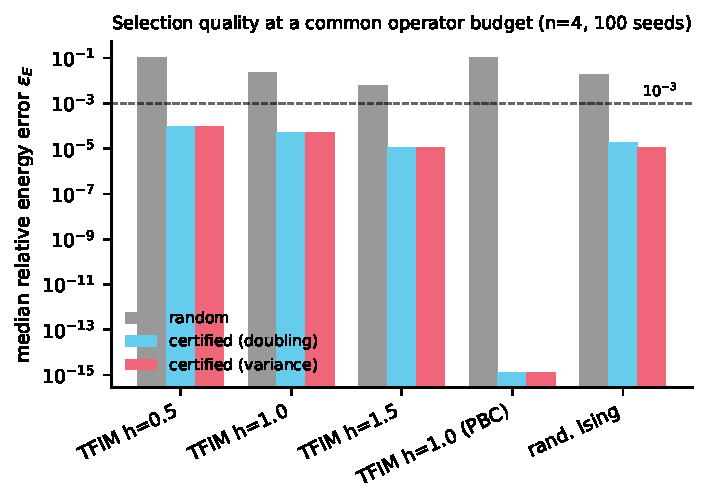
\includegraphics[width=0.99\columnwidth]{paper_assets/selection_quality.pdf}
\caption{Median relative energy error at a common eight-operator budget for random selection and two certified variants (uniform-doubling and variance-proportional allocation, both with QWC grouping), on five $n=4$ families, 100 seeds. The dashed line marks $\epsilon_E=10^{-3}$. The periodic-TFIM certified bars reach machine precision.}
\label{fig:selection}
\end{figure}

\begin{table}[t]
\caption{Headline $n=4$ selection, 100 seeds. $\epsilon_E$ is median relative energy error; $N_{\text{circ}}$ is median distinct measurement circuits; ``amb.'' is the fraction of selection steps ending budget-exhausted-ambiguous. Certified rows use QWC grouping.}
\label{tab:headline}
\centering
\begin{ruledtabular}
\begin{tabular}{llccc}
Family & Selector & $\epsilon_E$ & $N_{\text{circ}}$ & amb.\\
\colrule
TFIM $h{=}0.5$ & random & $1.1\times10^{-1}$ & 0 & ---\\
 & doubling & $9.1\times10^{-5}$ & 250 & 0.59\\
 & variance & $9.1\times10^{-5}$ & 220 & 0.35\\
\colrule
TFIM $h{=}1.0$ & random & $2.2\times10^{-2}$ & 0 & ---\\
 & doubling & $5.2\times10^{-5}$ & 283 & 0.79\\
 & variance & $5.2\times10^{-5}$ & 270 & 0.45\\
\colrule
TFIM $h{=}1.5$ & random & $5.9\times10^{-3}$ & 0 & ---\\
 & doubling & $1.1\times10^{-5}$ & 293 & 0.95\\
 & variance & $1.1\times10^{-5}$ & 287 & 0.70\\
\colrule
TFIM $h{=}1.0$ (PBC) & random & $1.1\times10^{-1}$ & 0 & ---\\
 & doubling & $1.4\times10^{-15}$ & 309 & 0.77\\
 & variance & $1.4\times10^{-15}$ & 306 & 0.39\\
\colrule
rand. Ising & random & $1.9\times10^{-2}$ & 0 & ---\\
 & doubling & $1.8\times10^{-5}$ & 280 & 0.67\\
 & variance & $1.1\times10^{-5}$ & 250 & 0.40\\
\end{tabular}
\end{ruledtabular}
\end{table}

\emph{QWC grouping.} Grouping the shared word set into commuting measurement bases leaves the estimator---and hence the median energy error and shot count---unchanged, while cutting the number of distinct circuits (Fig.~\ref{fig:grouping}). Across the five families the reduction is $3.1$--$4.0\times$: e.g., median circuits fall from 929 to 283 at the open critical point and from 1226 to 309 at the periodic point, where more commuting words are available to group. Because the certified doubling and grouped-doubling arms produce identical median errors ($5.2\times10^{-5}$ at the critical point in both cases), the circuit saving is free.

\begin{figure}[t]
\centering
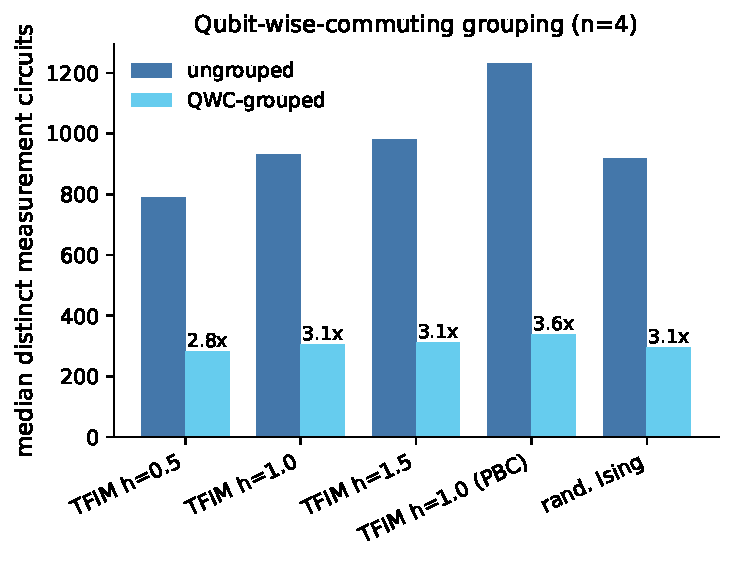
\includegraphics[width=0.85\columnwidth]{paper_assets/grouping.pdf}
\caption{Median distinct measurement circuits, ungrouped versus QWC-grouped, at fixed accuracy and shot budget ($n=4$, 100 seeds). Annotations give the reduction factor.}
\label{fig:grouping}
\end{figure}

\emph{Allocation.} Replacing uniform doubling by variance-proportional allocation reduces the fraction of selection steps that end ambiguous by $26$--$49\%$ (e.g., $0.79\to0.45$ at the critical point, $0.77\to0.39$ periodic), while holding or slightly improving the median energy error (Fig.~\ref{fig:allocation}). The improvement costs roughly twice the shots, because concentrating samples on the contested comparisons resolves more of them before the ceiling but does so by spending more total budget. Variance-proportional allocation is therefore the policy of choice when ambiguity, rather than raw shot count, is the binding constraint---for instance near reflection-symmetric points, where genuinely tied candidates are common (see below).

\begin{figure}[t]
\centering
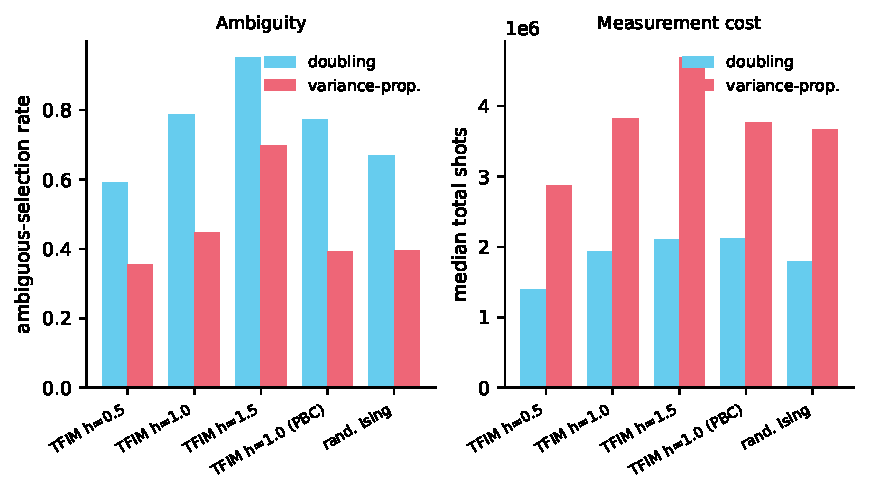
\includegraphics[width=0.99\columnwidth]{paper_assets/allocation.pdf}
\caption{Uniform-doubling versus variance-proportional allocation ($n=4$, 100 seeds, both grouped): (left) ambiguous-selection rate; (right) median total shots. Variance-proportional allocation lowers ambiguity at roughly twice the measurement cost.}
\label{fig:allocation}
\end{figure}

\emph{Scaling and pool expressivity at $n=6$.} On the 20-seed $n=6$ matrix, certified selection tracks the exact-gradient trajectory: on random-field Ising it reaches median relative error $4.1\times10^{-3}$ versus the exact selector's $4.5\times10^{-3}$, with near-optimal selection rate $0.96$, confirming that selection noise is not the accuracy bottleneck at this scale. The residual errors at $n=6$ are instead set by pool expressivity: on the XXZ chain even the \emph{exact} selector halts near $9.8\times10^{-2}$, because the two-local odd-$Y$ pool reaches an ADAPT gradient plateau---every remaining candidate gradient vanishes---before spanning the ground state. This cleanly separates selection quality from pool quality: the confidence machinery certifies the ranking, but certification cannot manufacture expressivity that the pool lacks. Random selection, by contrast, remains an order of magnitude worse ($6.7\times10^{-2}$ TFIM, $3.8\times10^{-1}$ XXZ), confirming that the gap of Fig.~\ref{fig:selection} persists with size.

\subsection{Molecular systems and the proxy--gradient boundary}
\label{sec:res-chem}

For fermionic chemistry a determinant-population proxy is a natural competitor: the FAST theory ranks excitations by sampled Slater-determinant populations rather than commutator gradients \cite{majland2023fast}, at one computational-basis circuit per step. We implement a FAST-inspired selector---scoring each candidate by a population-weighted Hamiltonian-connectivity term plus a determinant-pair coupling term---and compare it against exact and random selection on H$_2$, LiH (2e,\,2o), BeH$_2$ (4e,\,3o), and the H$_4$ chain, plus certified gradient selection on the three molecules small enough for it ($n\le6$; the H$_4$ chain uses eight qubits and is beyond the certified arm's protocol budget here), using the Jordan--Wigner singles-and-doubles odd-$Y$ pool (Fig.~\ref{fig:chem}, Table~\ref{tab:chem}).

At equilibrium geometry the small molecules are easy for every arm, and the proxy is dramatically cheaper: on BeH$_2$ the FAST-inspired selector reaches chemical accuracy in one operator using 4096 shots, against $1.69\times10^6$ shots for certified gradient selection---a $\sim\!410\times$ measurement saving---because a single determinant-population circuit suffices when the correlated correction is dominated by one excitation. This is the regime the FAST theory was designed for, and the operator-centric certified selector is not competitive on cost there.

The H$_4$ chain reverses the verdict. The FAST-inspired proxy fails \emph{deterministically}: its final error is $56.1$~mHa on all three seeds---worse than random selection ($10$--$19$~mHa)---and it never reaches chemical accuracy within the operator budget, while exact commutator-gradient selection reaches $0.42$~mHa in nine operators. Determinant populations are blind to the relative-phase structure that dominates the correlated H$_4$ state, so the proxy repeatedly selects the wrong excitation, and no number of shots corrects a signal that does not encode the gradient. Certified gradient selection, which estimates the correct observable, does not share this failure mode. The two arms thus bound the trade-off from both sides: the proxy is $\sim\!400\times$ cheaper when determinant structure carries the signal, and unboundedly wrong when it does not, whereas certified gradient selection pays more per step but never silently fails.

\begin{figure}[t]
\centering
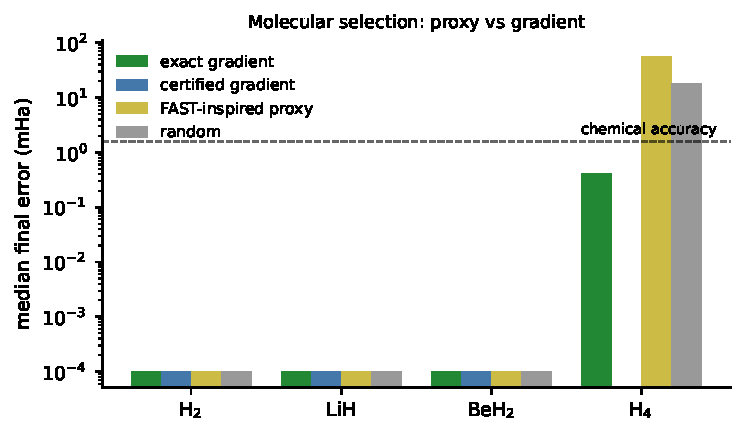
\includegraphics[width=0.95\columnwidth]{paper_assets/chemistry.pdf}
\caption{Median final energy error (mHa) by selection arm for four molecules; dashed line marks chemical accuracy. Equilibrium H$_2$/LiH/BeH$_2$ are solved by every arm---exact gradient, certified gradient, FAST-inspired proxy, and random---with bars clamped at the display floor. The certified-gradient arm is absent on the eight-qubit H$_4$ chain (beyond its protocol budget); there the FAST-inspired proxy fails deterministically at $56$~mHa---above random---while exact gradient selection reaches chemical accuracy.}
\label{fig:chem}
\end{figure}

\begin{table}[t]
\caption{Molecular selection. ``Err.'' is median final error (mHa); ``ops'' is operators to chemical accuracy (dash: not reached within budget); ``shots'' is median shots to accuracy. Confidence uses QWC grouping.}
\label{tab:chem}
\centering
\begin{ruledtabular}
\begin{tabular}{llccc}
Molecule & Selector & Err.\ (mHa) & ops & shots\\
\colrule
BeH$_2$ & exact & $0.0$ & 1 & 0\\
 & FAST & $0.0$ & 1 & $4.1\times10^{3}$\\
 & confidence & $0.0$ & 1 & $1.7\times10^{6}$\\
 & random & $0.0$ & 2--9 & 0\\
\colrule
H$_4$ & exact & $0.42$ & 9 & 0\\
 & FAST & $56.1$ & --- & ---\\
 & random & $18.1$ & --- & ---\\
\end{tabular}
\end{ruledtabular}
\end{table}

\subsection{Stabilizer-seeded initialization: a negative result}
\label{sec:res-stab}

Clifford-point initialization and stabilizer/residual splitting have been proposed to reduce the quantum work of variational solvers \cite{cheng2025clifford,robin2025stabilizer,yoo2025symmetry}. We tested whether a classically optimized stabilizer scaffold reduces the non-Clifford correction that adaptive selection must supply, using two variants: (A) discrete Clifford-point search over the HVA angles $\{0,\pi/2,\pi,3\pi/2\}$ evaluated on a stabilizer backend, and (B) a sign-consistent commuting-subset stabilizer approximation of $H$ whose ground state is prepared as a Clifford circuit and used as the ADAPT reference. The outcome is negative on every family tested. Variant A is vacuous for this ansatz class: the optimal Clifford point of the TFIM HVA \emph{is} the $\ket{+\cdots+}$ reference, verified by exhaustive enumeration through depth three. Variant B lowers the starting energy substantially---at $n=24$, $h=0.5$ the scaffold energy is $-23.0$ against the reference's $-12.0$, computed in a fraction of a second on the stabilizer backend---yet residual ADAPT from these scaffolds converges \emph{worse}: it reaches gradient plateaus with final relative errors $1.8\times10^{-2}$ to $3.3\times10^{-2}$ on the open and periodic critical TFIM and four of five disorder realizations, against $\le10^{-4}$ for the unseeded baseline. The lone partial positive is the ordered phase, where the $h=0.5$ scaffold reaches $10^{-2}$ relative error in six operators against the baseline's eight. The predictor of correction cost is thus not the scaffold energy but the alignment of the reference with the ground-state symmetry sector: the $X$-field reference sits in the correct parity sector and the $Z$-cluster scaffold does not. We therefore report stabilizer seeding as a negative result rather than an independent method; the machinery (stabilizer backend, Clifford-point search, stabilizer approximation) is retained as reproducible infrastructure.

\section{Discussion}
\label{sec:discussion}

The operator-centric language earns its place where it makes selection structure explicit. Because every $G_j$ is a Hermitian multivector over the same Pauli basis as $H$, the union word set \eqref{eq:wordset} and the candidate-by-word matrix are immediate, and global measurement reuse is a property of the data structure rather than a bespoke optimization. The transpose-parity rule (Proposition~\ref{prop:oddy}) is likewise a one-line consequence of transposition being diagonal on Pauli words, and it removes half the candidates before any shot is taken. Certification then rides on the same representation: the estimator, its variance, and the simultaneous bounds are computed from the shared cache without a change of type.

The results delineate three regimes. When the pool is expressive and the state is generic, certified gradient selection is decisively better than random and never worse than the exact selector's trajectory up to the reported confidence (Sec.~\ref{sec:res-spin}). When a cheap proxy encodes the relevant signal---dominant determinant populations in equilibrium chemistry---the proxy wins on cost by orders of magnitude, and a gradient method should defer to it (Sec.~\ref{sec:res-chem}). When the proxy's signal and the true gradient diverge, as in the correlated H$_4$ chain, the proxy fails silently and unboundedly while certification does not. A practical adaptive solver should therefore treat proxy and certified gradient selection as complementary and diagnose which regime it is in, rather than committing to one globally.

Our framework is complementary to, and composable with, the measurement-reduction literature. Commuting-gradient measurement \cite{anastasiou2023gradients} and Pauli-outcome reuse with variance allocation \cite{ikhtiarudin2025shot} reduce the cost of estimating a fixed set of gradients; the global bank and QWC grouping here extend reuse across the \emph{whole} pool and across allocation rounds; and best-arm racing decides which candidates should keep receiving shots at a fixed ceiling. Layering and subpool exploration \cite{long2024layering} act on a different axis (depth and processor calls) and could be layered on top. A natural next system groups commuting words, reuses compatible outcomes across candidates and iterations, and races candidates under covariance-aware, empirical-Bernstein confidence regions---each ingredient present here in isolation.

\section{Limitations}
\label{sec:limitations}

The numerical claims are deliberately bounded. First, $n\le6$ (spin) and four-qubit-scale active spaces (chemistry) verify correctness and qualitative behavior but do not establish favorable scaling; we claim no quantum advantage, and the dense eigensolver remains the validation backend. Second, only ADAPT selection is sampled: optimizer shot noise, device decoherence, state-preparation and measurement error, and compilation constraints are absent. Third, the robust confidence tier uses a normal approximation with a \v{S}id\'ak correction and inherits winner-selection bias; the empirical-Bernstein tier is provided but the reported experiments use the robust tier, so the stated $\delta$ is a design target rather than a proven familywise guarantee under adaptive stopping. Fourth, per-word variances ignore cross-word covariance within a QWC group, which is conservative for the reconstruction \eqref{eq:bankest} but not exploited; correlated estimators such as classical shadows \cite{huang2020shadows} could lower the effective cost further. Fifth, the pools are problem-specific greedy choices; exact reoptimization guarantees a monotone variational energy but cannot refund a poor slot or the shots spent selecting it, and the XXZ result shows that certification does not substitute for an expressivity analysis. Finally, the FAST-inspired arm is a faithful-in-spirit reimplementation, not the original FAST estimator, so the chemistry comparison bounds a mechanism (population proxy versus gradient) rather than a specific published implementation.

\section{Conclusion}

We have built finite-shot ADAPT operator selection as a certified statistical procedure inside a sparse operator-centric Clifford algebra, in which all commutator-gradient observables live in one shared Pauli-word basis. A global commutator bank and cumulative cache pay for each shared word once; QWC grouping collapses the cache to one circuit per commuting group, cutting distinct measurement circuits by $3.1$--$4.0\times$ at unchanged accuracy; and a best-arm selector with simultaneous confidence bounds reports an explicit four-way outcome, controlling the probability of a wrong selection instead of silently guessing. Across five spin families at $n=4$ (100 seeds) certified selection beats random by two to more than three orders of magnitude at a fixed operator budget, and variance-proportional allocation halves the ambiguous-selection rate. On molecules the framework maps the exact boundary at which a determinant-population proxy fails---$\sim\!400\times$ cheaper than gradient selection on equilibrium BeH$_2$, but deterministically wrong on the correlated H$_4$ chain where gradient selection still converges. Stabilizer-seeded initialization is reported as a negative result: scaffold energy does not predict the non-Clifford correction cost, symmetry alignment does. Together these provide a reproducible, algebraically unified baseline for measurement-limited adaptive eigensolvers, and a concrete diagnosis of when finite-shot selection can be certified and when no amount of measurement will help.

\appendix

\section{Confidence construction and selection outcomes}
\label{app:confidence}

With active candidate set of size $m$ and per-word cache $(N_w,k_w)$, the Jeffreys mean and variance are $\widetilde m_w=2(k_w+\tfrac12)/(N_w+1)-1$ and $\widehat\Var(\widehat m_w)=(1-\widetilde m_w^2)/(N_w+1)$; a word never measured contributes mean $0$ and variance $+\infty$, so untouched candidates stay maximally uncertain. Candidate reconstruction is Eq.~\eqref{eq:bankest}. The simultaneous radius \eqref{eq:radius} spends the error budget across candidates by \v{S}id\'ak and across a geometric round schedule by a union bound, so the per-round, per-candidate level is $1-(1-\delta/R)^{1/m}$ for $R$ planned rounds. A step returns \textsc{below\_threshold} when every candidate's upper bound is under the gradient threshold; \textsc{resolved\_best} when Eq.~\eqref{eq:resolve} holds above threshold; \textsc{resolved\_near\_optimal} when the leader clears threshold and the residual gap to the runner-up is within $\varepsilon$; and \textsc{budget\_exhausted\_ambiguous} otherwise. The empirical-Bernstein radius $\sqrt{2\widehat v\ln(3/\delta)/N}+3R_{\mathrm{range}}\ln(3/\delta)/N$ \cite{maurer2009empirical}, with $R_{\mathrm{range}}=2$ for $\pm1$ outcomes, is available as a drop-in replacement valid under data-dependent stopping.

\section{Reproducibility}
\label{app:repro}

The replication package contains the NumPy-only algebra kernel and Pauli-rotor IR, the exact and finite-shot backends, the commutator bank, cache, confidence, and allocation modules, the selection algorithms, the model builders (spin and molecular), adversarial regression tests, and the committed per-seed benchmark records with their summary tables and figure script. Each benchmark regenerates from a single command with predeclared seeds, budgets, tolerances, and confidence level; long sweeps shard across workers. Figure values are read from the committed records rather than transcribed. The maintained public project is at \url{https://github.com/gutama/clifford_qc}; the submission-associated revision is intended to be released as a tagged version.

\bibliographystyle{apsrev4-2}
\bibliography{references}

\end{document}
